\chapter*{Introduction}
\addcontentsline{toc}{chapter}{Introduction}

Introduce the problem, explain why it is interesting and outline the goal of the thesis.

\begin{itemize}
\item Introduce the problem
\item Describe what has already been done
\item {\bf Emphasize what we want to achieve}
\item Mention the structure of the thesis
\end{itemize}

More in detail:

\begin{itemize}
\item The problem is that current visualization methods in Morphome3cs which work with homologous meshes are not sufficient.
\item Various metrics are being visualized by vertex color. Also mention related difference visualizations and that they all solve a slightly different problem (no homologous meshes) and mostly also just use color.
\item {\bf The goal is to come up with a good arrow-based visualization and experiment with the visual appearance to get a satisfactory result.}
\item (Thesis structure)
\end{itemize}

\section*{Morphome3cs}

\section*{Applications of Mesh Difference Visualization}
%%-----------------------------------------------------------------------------------------
%%-----------------------------------------------------------------------------------------
\section*{Mesh Difference Visualization in Morphome3cs and Elsewhere}

Morphome3cs is able to generate a homologous\footnotemark pair of triangle meshes from two arbitrary meshes and uses it to compute and visualize the difference. Currently, Morphome3cs is able to produce color-based visualizations of multiple difference metrics. These metrics are:

\begin{itemize}
\item Vertex distance (fig. \ref{fig:morpho_example})
\item Vertex distance projected into the surface normal
\item Angle between corresponding surface normals
\item FESA\footnotemark
\item Curvature difference
\end{itemize}

The disadvantage of these color-based visualizations is that they fail to capture multi-dimensional information. For example, when using vertex distance as a metric, it is impossible to encode both magnitude and direction into color at the same time while maintaining visual clarity.

\begin{figure}[h]
\centering
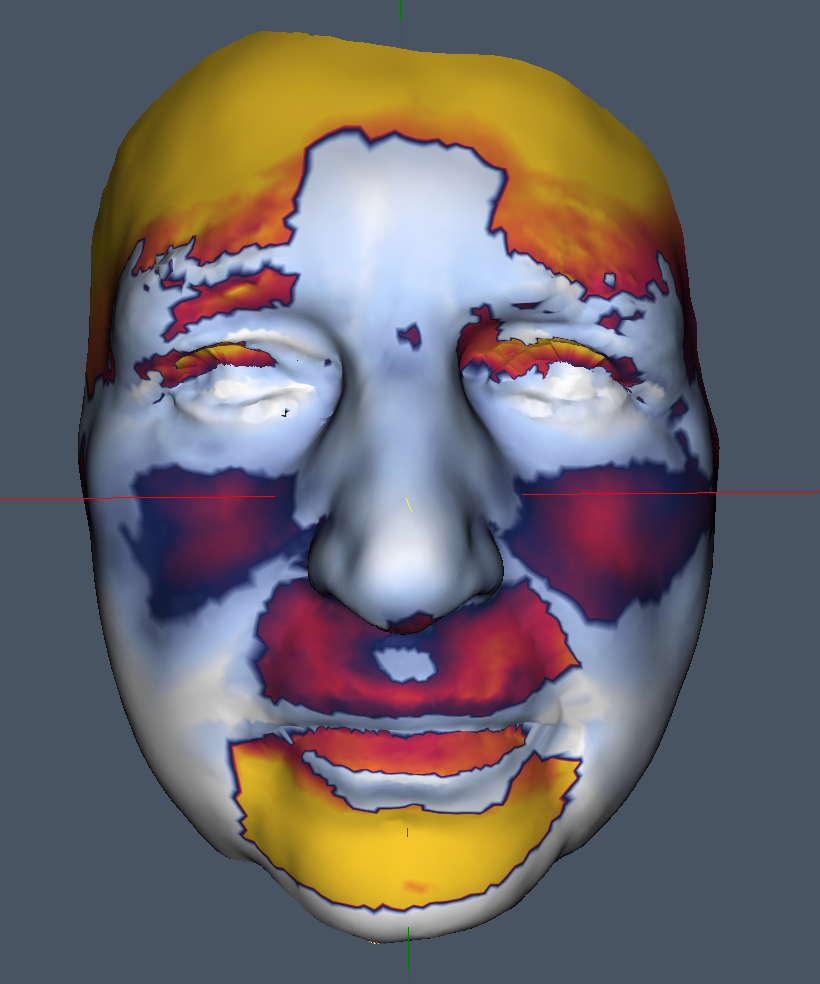
\includegraphics[width=0.5\textwidth]{./img/morpho-example01.PNG}
\caption{Morphome3cs - Vertex difference visualization}
\label{fig:morpho_example}
\end{figure}

Other approaches can be found for example in MeshLab (fig. \ref{fig:meshlab_example}) and CloudCompare (fig. \ref{fig:cloudcompare_example}). Both programs, however, also use only color-based visualizations. Both programs work with arbitrary triangle meshes and CloudCompare can also work with point clouds, register them and visualize the difference between them.

\begin{figure}[h]
\centering
	\begin{subfigure}{0.3\textwidth}
	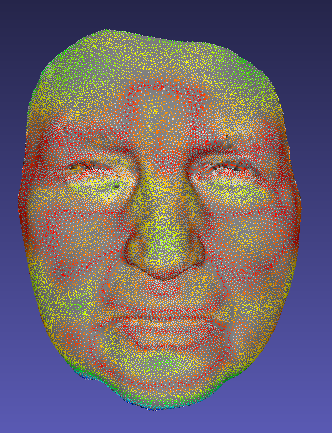
\includegraphics[width=\textwidth]{./img/meshlab-example01.PNG}
    \caption{MeshLab - Hausdorff Distance visualization}
    \label{fig:meshlab_example}
	\end{subfigure}
    \qquad
    \begin{subfigure}{0.3\textwidth}
	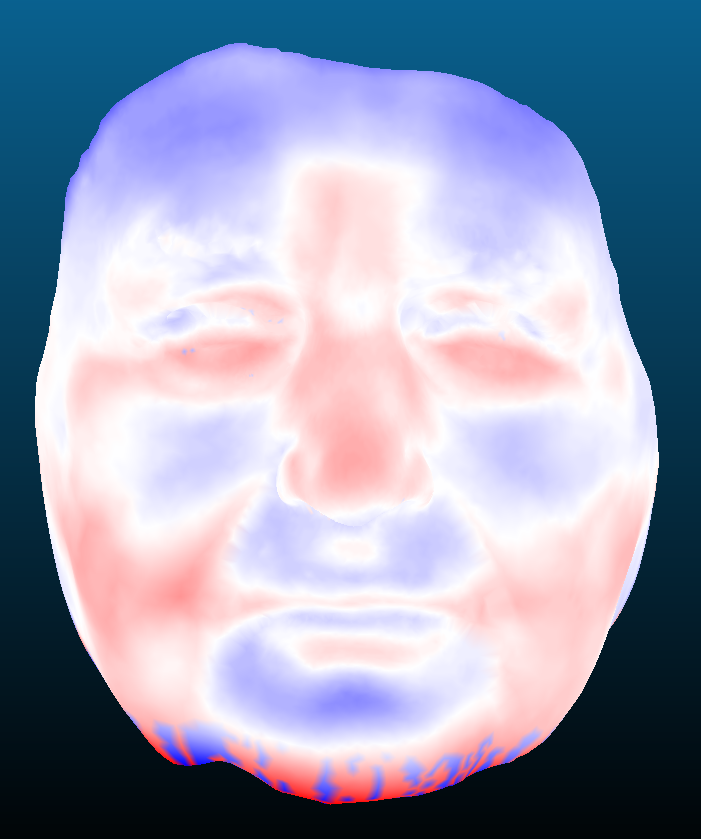
\includegraphics[width=\textwidth]{./img/cloudcompare-example01.PNG}
    \caption{CloudCompare - Vertex distance visualization}
    \label{fig:cloudcompare_example}
	\end{subfigure}
\caption{Visualizations in MeshLab and CloudCompare}
\end{figure}

\addtocounter{footnote}{-2}
\stepcounter{footnote}\footnotetext{Two triangle meshes are homologous if they have the same number of vertices and there is a one-to-one mapping between them. Vertices are numbered and vertex \(v_i \in Mesh_1\) corresponds to vertex \(v_i \in Mesh_2\).}
\stepcounter{footnote}\footnotetext{{\it Finite Element Surface Analysis}, captures the difference between corresponding triangle areas}
%%-----------------------------------------------------------------------------------------
%%-----------------------------------------------------------------------------------------
\section*{Our Goal}

\section*{Thesis Structure}